\documentclass[10pt,a4paper]{article}
\usepackage[utf8]{inputenc}
\usepackage[french]{babel}
\usepackage[T1]{fontenc}
\usepackage{amsmath}
\usepackage{amsfonts}
\usepackage{amssymb}
\usepackage{graphicx}
\usepackage{hyperref}
\usepackage[left=2cm,right=2cm,top=2cm,bottom=2cm]{geometry}
\usepackage{siunitx}
\author{Baptiste Rouger}
\title{Lab Notebook MSC}

\setcounter{secnumdepth}{0}

\begin{document}
\maketitle

\tableofcontents

\newpage

\section{15 Jan 2018}

\begin{itemize}
        \item Début d'installation sur le PC
        \item Cassage de ArchLinux
        \item Rangement de la salle de manip et mise en place de la salle de manip
                \begin{itemize}
                        \item Raccourcissement des plus longues barres de la cage qui gênaient.
                        \item Réorganisation de la salle
                \end{itemize}
        \item Lecture de la review de Mathieu
\end{itemize}
\noindent Comment la température ambiante influence la fermeture des feuilles? \\
Comment la fermeture des feuilles affecte la température de celles-ci?

\section{16 Jan 2018}
\begin{itemize}
        \item Installation de Debian sur le PC
        \item Installation des logiciels importants sur le PC
        \item Mise en place de la première manip test pour la \textbf{nutation}: début à \textbf{15h52}, fin à \textbf{10h42} le 17 Jan 2018. Les données sont situées sur Alfred: /mnt/data/manip/Baptiste/test\_16-01-2018.J'ai utilisé la plante "Abby" pour réaliser cette manip. Photo toutes les 90 secondes.
\end{itemize}

\section{17 Jan 2018}
\begin{itemize}
        \item Arrêt de la manip \textbf{test\_16-01-2018} à \textbf{10h42}
        \item Arrosage des plantes
        \item Récupération des données de la manip
        \item Création du film à partir des données de la manip (\textit{cf}\textsc{Protocole}~\ref{film})
        \item Réalisation du script \textbf{analysisScript.py} qui, à partir de photos stockées dans un dossier, réalise la timeline d'une ligne de pixel et la converti en image binaire
\end{itemize}

Le lien pour la vidéo: \url{http://uptobox.com/5x80eimcd7xu}\\

Le résultat du script \textbf{analysisScript.py} :\\

\includegraphics[width = \linewidth]{imTLBWv1.jpg}

\section{18 Jan 2018}
\begin{itemize}
        \item Début d'une deuxième manip pour observer la nutation (sur un plus long terme). Début à environ 12h30 \textbf{(heure pc décalée????)}. Il fait \SI{24.2}{\celsius} dans la pièce, 49\% d'humidité. On utilise la plante "Béa". Les numéro de protocole sont:
                \begin{itemize}
                        \item arduino: 21608
                        \item photos: 21821
                \end{itemize}
        \item Création du script appelé \textbf{anSc3.py} qui utilise la librairie skimage pour analyser les images et réaliser le graphe de mouvement.

\end{itemize}

\section{19 Jan 2018}
Je me suis penché sur le problème du maintien de la température et de l'humidité de la salle de manip avec Arduino (ainsi que la photopériode). J'ai pris en compte la mesure de ces données. Schéma :\\
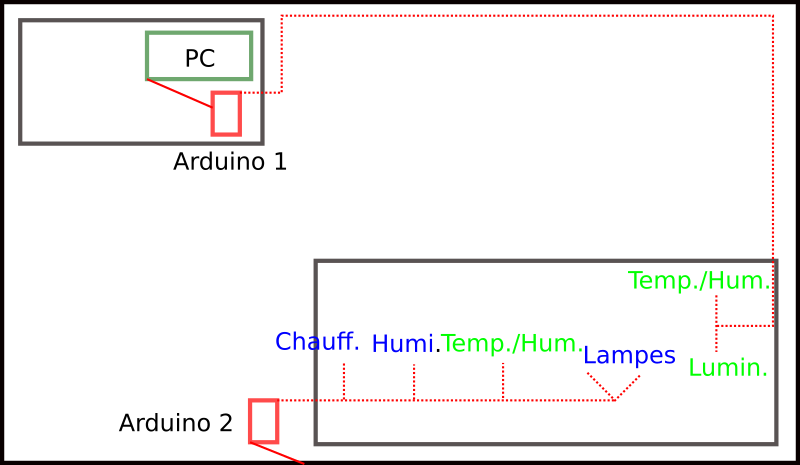
\includegraphics[width=0.6\linewidth]{schema_Arduino.png}

\section{20 Jan 2018}
J'ai refait le focus sur la jeune feuille, il n'était évidemment plus bon au bout de ces 2 jours et demi. $\Rightarrow$ Il serait intéressant de voir si l'auto focus pourrait compenser intelligemment cela.\\

Pour les scripts, je vais essayer de trouver la position du centre de la tige en utilisant une moyenne pondérée par le nombre de pixels consécutifs\\

J'ai modifié les scripts : je les ai séparé en deux : \texttt{TL.py} sert à créer l'image de la timeline, \texttt{Trajec.py} sert à récupérer la position moyenne de la tige. On peut entre les deux scripts retailler l'image.

\section{29 Jan 2018}
J'ai travaillé sur les scripts d'analyse de l'image, de récupération de la trajectoire et d'analyse en ondelette de ces trajectoires. J'ai découpé chaque étape et je les ai mises dans des scripts précédents qui prennent différents arguments (\textit{cf} \textsc{Protocole}~\ref{anaNut}).

J'ai fini le robot arduino qui contrôle la température, l'humidité et les lampes. Je le teste pour la nuit.

\section{30 Jan 2018}

Il y avait un problème dans le robot de contôle. J'ai dû modifier le code d'une part (problème de LOW et HIGH en output pour les relais). De plus, j'ai dû installer la librairie Time sur le pc de la salle de manip. J'ai vérifié que cela fonctionnait bien quelques minutes. Le nouveau code arduino pour le robot est joint dans le dépôt : \texttt{arduino\_Stat.ino}.\\

J'ai remarqué que la lampe numéro 2 (au dessus de la cage) ne fonctionne plus.

\section{31 Jan 2018}
Le robot de contrôle était encore bugé. Il se trouve que les relais se bloquent parfois et restent en position de contact alors qu'ils devraient couper le courant. Cela n'arrive que quand on branche la grosse lampe. Peut-être tire-t-elle trop de courant pour notre carte de relais. Il faudra voir si la carte est théoriquement capable de supporter les intensités que nous lui faisons traverser.\\

J'ai également retravaillé les codes d'analyse d'images. Ils sont toujours découpés en trois parties, mais maintenant on peut spécifier plusieurs lignes à \texttt{1-TL.py} pour éviter d'avoir à relancer le process des images trop de fois. Par ailleurs, j'utilise maintenant numpy.savetxt pour sauver la trajectoire en csv dans \texttt{2-Traj.py}, ainsi que numpy.loadtxt pour la charger dans \texttt{3-WL.py}. J'ai aussi nettoyé le code de tous les commentaires de débugage inutiles.

\section{01 Fev 2018}
Le robot de contrôle semble avoir grillé la lampe d'aurore ! De plus, il semble qu'avec le temps l'horloge de l'arduino se décale. Je vais essayer de voir de combien en combien de temps. Pour cela, j'ai pris un screen avec l'heure de l'arduino et l'heure du PC. Celui-ci se situe dans le dossier Pictures de manip.





\newpage
\begin{center}
        {\Huge Protocoles}
\end{center}
\appendix

\section{Creation du film à partir des images\label{film}}
\begin{enumerate}
        \item On utilise Thunar pour renommer nos fichier pour que leurs noms soient une suite numérotée ininterrompue (eg. 001.jpg, 002.jpg, etc)
        \item On utilise la commande \texttt{ffmpeg -framerate 40 -i \%03d.jpg -c:v libx264 -profile:v high -crf 20 -pix\_fmt yuv420p output.mp4}
\end{enumerate}
Les fichiers à utiliser sont données par l'option \texttt{-i}, on peut changer le framerate (ici 40 images par secondes).

\section{Analyse des images de la nutation\label{anaNut}}
\begin{enumerate}
    \item On a mis toutes les photos du film dans un dossier. On récupère le chemin d'accès à ce dossier.
    \item On utilise la commande : \texttt{python 1-TL.py Path Lines} avec \texttt{Path} est la localisation du dossier \texttt{Line} est une suite de lignes de pixel à extraire des photos (e.g. 500,600,700 sans espace, séparés par des virgules)
    \item Puis \texttt{python 2-Traj.py Path Picture dt} avec \texttt{Path} la localisation du dossier, \texttt{Picture} est le nom de l'image générée par \texttt{1-TL.py}, et \texttt{dt} est le temps entre chaque photo.
    \item Enfin \texttt{python 3-WL.py Path CSV} avec \texttt{Path} la localisation du dossier, \texttt{CSV} le nom du fichier csv créé par \texttt{2-Trajec.py}
\end{enumerate}




\end{document}
